\usetikzlibrary{calc}
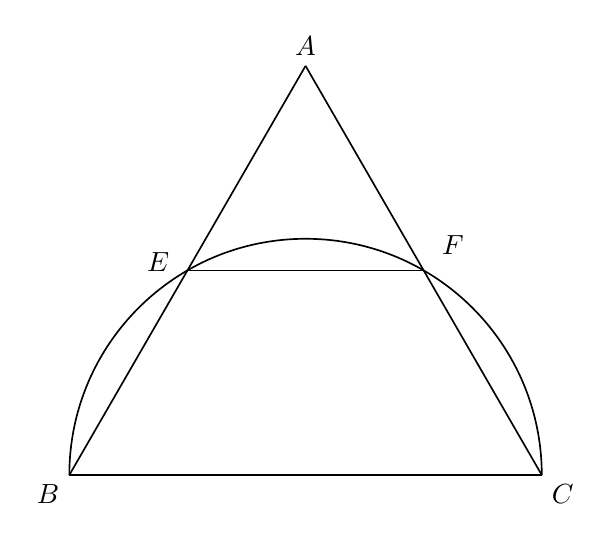
\begin{tikzpicture}[x=1cm,y=1cm,line width=.6pt,font=\normalsize]
\coordinate (B) at (0,0);
\coordinate (C) at (6,0);
\coordinate (O) at (3,0);
\coordinate (A) at (3,5.1961524227);
\coordinate (E) at (1.5,2.5980762114);
\coordinate (F) at (4.5,2.5980762114);
\draw (B)--(C);
\draw (A)--(B);
\draw (A)--(C);
\draw (E)--(F);
\draw (B) arc[start angle=180,end angle=0,radius=3cm];
\node[above] at (A) {$A$};
\node[below left] at (B) {$B$};
\node[below right] at (C) {$C$};
\node[left,xshift=-3pt,yshift=3pt] at (E) {$E$};
\node[above right,xshift=3pt,yshift=2pt] at (F) {$F$};
\end{tikzpicture}
